\chapter{Reconstruction}
\label{ch:reconstruction}

Each event within an AD was assigned a reconstructed position and energy
that accounted for the pattern of PMT hits, the total light emitted,
scintillator and mineral oil optical characteristics,
spatial nonuniformity, and electronics nonlinearity.
The reconstructed positions were used to compute the distance-time cut
to select IBD events as described in \cref{sec:DT_cut},
and were also used as inputs to the energy reconstruction
to help correct for nonuniformities in the ADs' light collection
as a function of position.
The reconstructed energy was a critical input to the \thetaot{} analysis
due to the heavy reliance on energy cuts to select IBDs and reject background.
The relative performance of ADs in reconstructing energy
was particularly important, since inconsistencies in energy reconstruction
could lead to unaccounted-for differences in efficiency,
which would bias the measurement of \thetaot.
The position reconstruction procedure will be detailed in \cref{sec:reco_position}.
Energy reconstruction, including the energy scale, determination of event energy,
and the nonuniformity and nonlinearity corrections,
will be described in \cref{sec:reco_energy}.

\section{Position}
\label{sec:reco_position}

Daya Bay used two independent position reconstruction algorithms,
both of which relied on the pattern of charge measurements across all PMTs in an AD.
The reconstruction used in this \thetaot{} analysis is known as ``AdSimple;''
the name was inherited from a predecessor algorithm \cite{adsimple1}.
The other reconstruction is called ``AdScaled.''

In AdScaled, a center-of-charge position was computed,
averaging over each PMT position weighted by the charge on the PMT,
and a parametrized correction derived from simulation
was applied to determine the reconstructed position \cite{ngd2016}.
However, AdSimple was determined to be the better algorithm for use in the nH analysis
\cite{adsimple_vs_adscaled_nh}.

In AdSimple,
each event's PMT charge pattern was compared to a library of \num{9600} templates
generated using a Monte Carlo simulation.
Each template represented one position on an $(r, \phi, z)$ grid
with \num{20} $r$ positions, \num{24} $\phi$ positions,
and \num{20} $z$ positions.
A $\chi^2$ was constructed to quantify the agreement between the measured charge pattern
and each of the templates:
\begin{equation}
    \chi^2(\textbf{r}_{\text{rec}}) = \sum_{i=1}^{192} -2\ln\frac{
        \text{Poisson}(N_i^{\text{obs}} \vert N_i^{\text{template}}(\textbf{r}_{\text{rec}}))
    }
    {
        \text{Poisson}(N_i^{\text{obs}} \vert N_i^{\text{obs}})
    },
\end{equation}
where $i$ indexes over PMTs,
$N_i^{\text{obs}}$ is the number of photoelectrons observed in PMT $i$,
$N_{i}^{\text{template}}(\textbf{r}_{\text{rec}})$ is the prediction
for PMT $i$ of the template for reconstructed position $\textbf{r}_{\text{rec}}$,
and $\text{Poisson}(n\vert\mu)$ is the Poisson probability
to observe $n$ counts given an expected value of $\mu$.
Once the lattice point with the least $\chi^2$ was found,
an interpolation was performed along each coordinate dimension $(r, \phi, z)$
as depicted in \cref{fig:interpolation}
to extend the domain of the $\chi^2$ function to all positions within the AD,
not just the lattice points.
The value of $\textbf{r}_{\text{rec}}$ which minimized $\chi^2$
was used as the reconstructed position.
The distribution of reconstructed positions
for all single and double coincidences in EH1-AD1
is shown in \cref{fig:position_map};
the distribution was qualitatively identical in all ADs.
The grid pattern in the distribution is an artifact of the interpolation process.
The maximum reconstructed radius displayed is \SI{2.2}{\m}
due to the flasher cuts described in \cref{sec:flashers}.

\begin{figure}
    \centering
    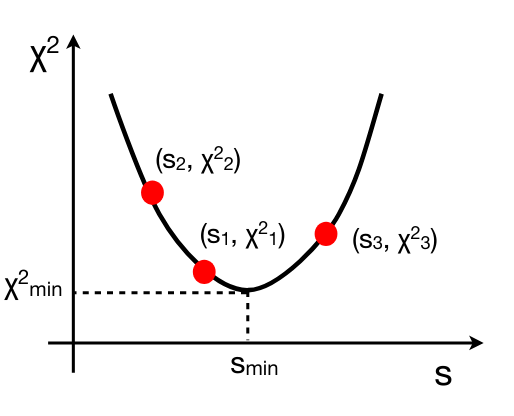
\includegraphics[width=0.4\textwidth]{ch_reconstruction/interpolation}
    \caption[Position reconstruction interpolation]{
        Interpolation between grid points to obtain a more-precise position
        that minimizes the $\chi^2$ function.
        The process is repeated with $s$ representing each of the coordinates
        $r, \phi, z$.
        Figure taken from \cite{adsimple1}.
    }
    \label{fig:interpolation}
\end{figure}

\begin{figure}
    \centering
    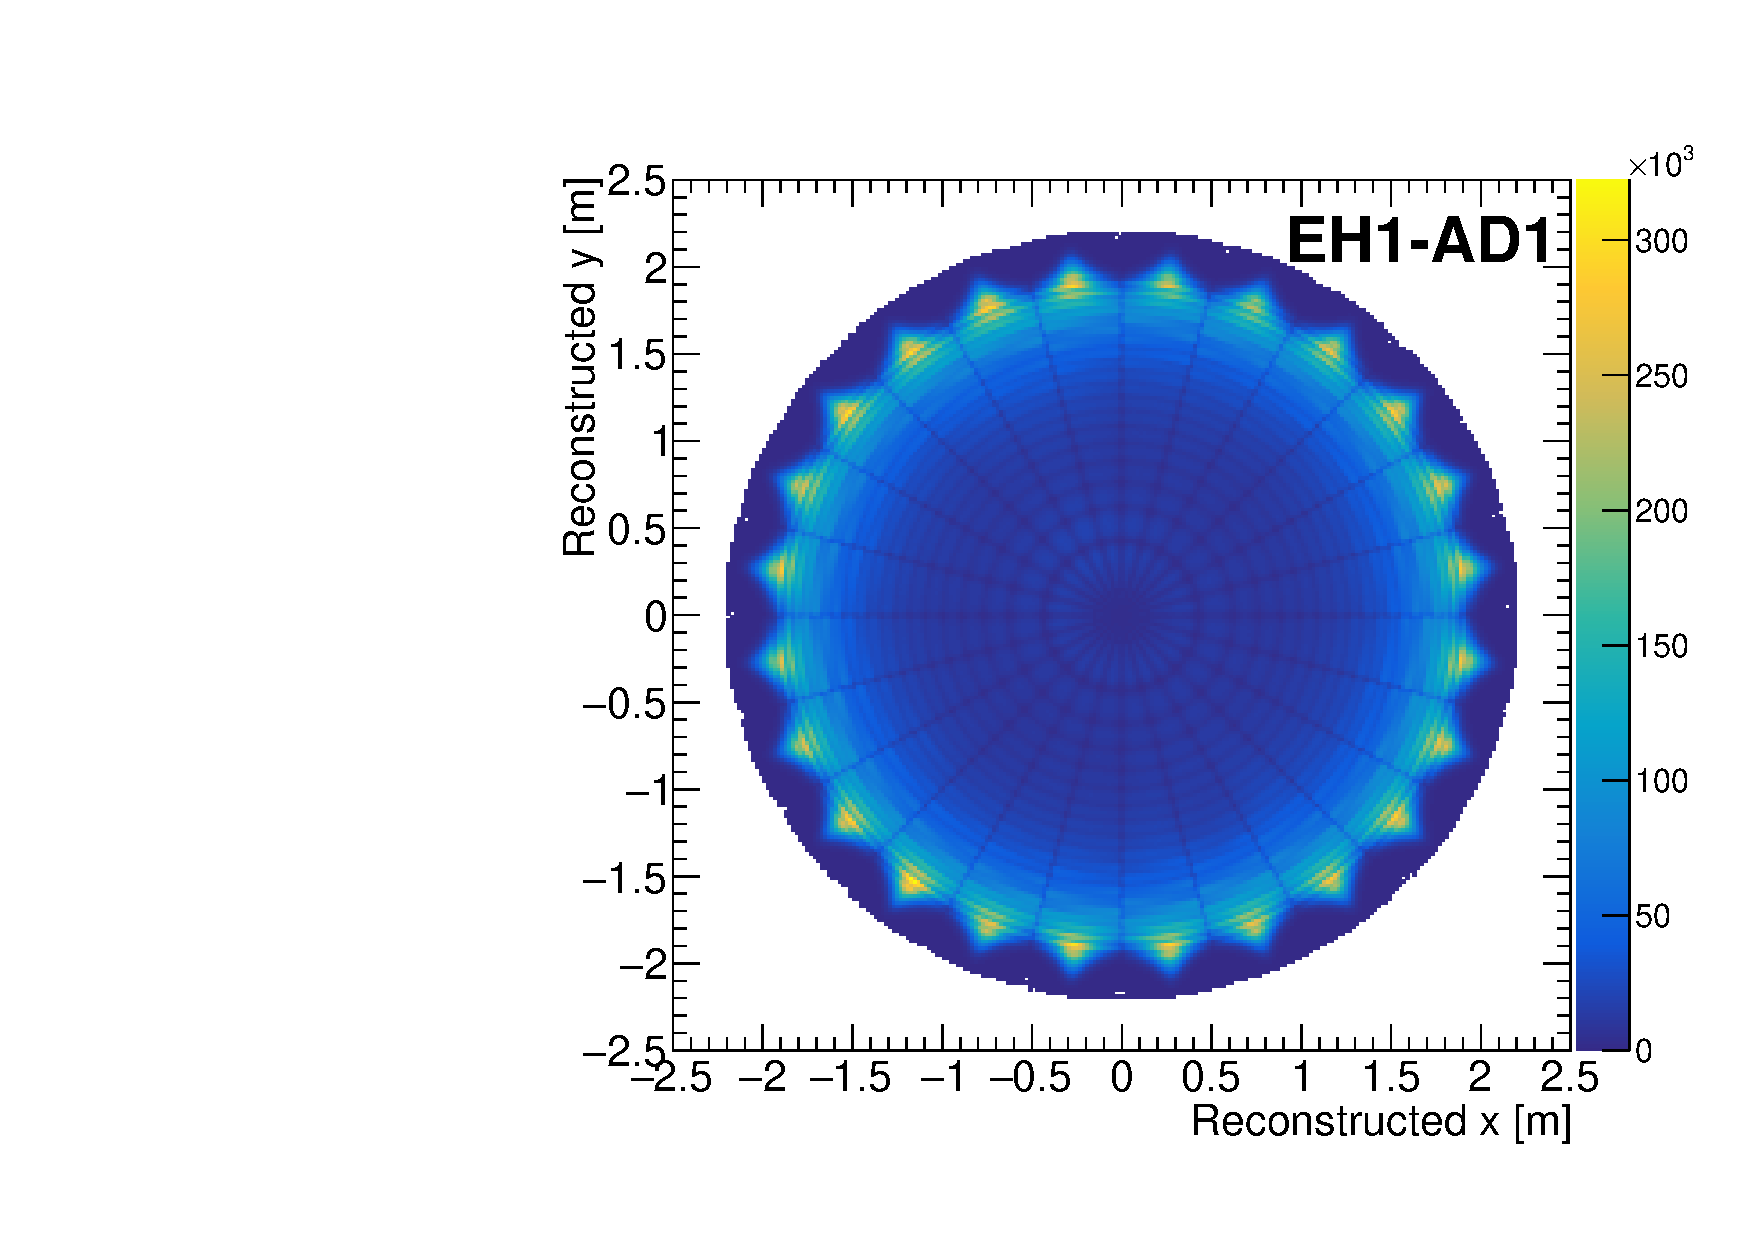
\includegraphics[width=0.8\textwidth]{ch_reconstruction/xy}
    \caption[Reconstructed position distribution]{
        Reconstructed positions of single and double coincidence events
        with energy within \SIrange{1.5}{12}{\MeV} in EH1-AD1.
    }
    \label{fig:position_map}
\end{figure}

\section{Energy}
\label{sec:reco_energy}

The reconstructed energy for an event was built up from the previously-described
calibration values and the observed signals in each PMT.
PMT observed ADC values were converted into charges using the gain
and corrected for the single-channel nonlinearity (\cref{subsec:scnl}).
The total charge on all PMTs was converted into an energy value
using the light yield measured during calibration,
and then corrected to account for any disabled PMTs
and for variations in the detector response as a function of position and time.
This process can be represented by the following formula:
\begin{equation}
    E_{\text{rec}} = \left(
        \sum_i f_{\text{SCNL}}\left(\frac{Q_i}{\overline{Q}_i^{\text{SPE}}(t)}\right)
    \right)
    \frac{f_{\text{act}}(t)}{N^{\text{PE}}(t)}
    f_{\text{pos}}(\textbf{r}_{\text{rec}},t),
\end{equation}
where $Q_i$ is the ADC value for PMT $i$,
$\overline{Q}_i^{\text{SPE}}(t)$ and $N^{\text{PE}}(t)$
are the gain for PMT $i$ and the light yield, respectively
(\cref{sec:gain,sec:light_yield_calib}),
$f_{\text{SCNL}}$ is the single-channel nonlinearity correction
(\cref{subsec:scnl}),
and $f_{\text{act}}(t)$ and $f_{\text{pos}}(\textbf{r}_{\text{rec}},t)$
are the active PMT correction and nonuniformity correction,
described below.

The active PMT correction compensated for the loss in collected light
when a PMT was disabled during operation \cite{ngd2016}.
On average, each PMT contributed $\nicefrac{1}{192}$ of the charge to each event.
Thus if $n$ PMTs were disabled, the apparent measured total charge must be increased by a factor
\begin{equation}
    f_{\text{act}}(n) = \frac{192}{n}.
\end{equation}
The correction was time-dependent since the number of disabled PMTs changes with time.

The rest of this chapter will describe the
nonuniformity correction $f_{\text{pos}}(\textbf{r}_{\text{rec}},t)$
(\cref{subsec:nonuniformity})
as well as characterizations of the detector energy response:
the energy resolution (\cref{subsec:resolution}),
relative energy scale (\cref{subsec:rel_energyscale}),
and absolute energy scale (\cref{subsec:abs_energyscale}).

\subsection{Nonuniformity correction}
\label{subsec:nonuniformity}

The nonuniformity correction ensured that events of a given physical energy
occurring in different regions of the AD
were assigned the same reconstructed energy.
Nonuniformities in reconstructed energy arose due to a variety of factors
including PMT light acceptance as a function of incident angle;
optical properties of the scintillator, mineral oil, and acrylic vessels;
and the orientation of PMTs with respect to the Earth's magnetic field.
The nonuniformity correction was factored into corrections based on
$r$ and $z$ position, azimuthal angle $\phi$, and time:
\begin{equation}
    f_{\text{pos}}(\textbf{r}_{\text{rec}},t) =
    f_{\text{pos}}(r, z)f_{\text{pos}}(\phi)f_{\text{pos}}(r, t).
\end{equation}

Maps for the $r$--$z$ nonuniformity were constructed for each AD
by identifying neutron captures on both Gd and H,
and comparing the energy of events in a given region of the AD
to the average of the entire AD.
The AD was divided into equal-volume concentric rings
represented as squares on a plot of $z$ vs. $r^2$.
Neutron captures of spallation neutrons were selected
based on a time coincidence with a previous muon signal in the AD.
Neutron captures with energy near \SI{8}{\MeV} were assumed to be nGd captures,
and those with energy near \SI{2.2}{\MeV} were assumed to be nH.
The peak value was extracted from a fit of the respective distributions
for each pixel and for the entire sample.
The nGd peak was fit with a double-Crystal Ball function \cite{cbfunction}
(described in \cref{sec:light_yield_calib})
and used to characterize pixels within the GdLS volume.
The nH peak was fit with a calorimeter function \cite{calorimeter2016}
(described in \cref{subsec:delayed})
and used for the pixels within the LS volume.
A correction was then constructed to apply to each event's energy based on its position:
\begin{equation}
    f_{\text{pos}}(r, z) = \frac{E_{\text{avg}}}{E_{\text{pixel}}(r,z)},
\end{equation}
where $E_\text{avg}$ is the average fitted peak energy over all pixels,
and $E_\text{pixel}(r, z)$ is the fitted peak energy for the pixel
containing the point $(r, z)$.
\Cref{fig:nonuniformity_map} shows the corrections $f_{\text{pos}}$ for EH1-AD1.
All ADs had similar nonuniformities, but separate corrections were still computed
for each AD.
Within an AD, the nonuniformity correction was as large as \SI{20}{\percent}
at the outer edge of the OAV (LS region).

\begin{figure}
    \centering
    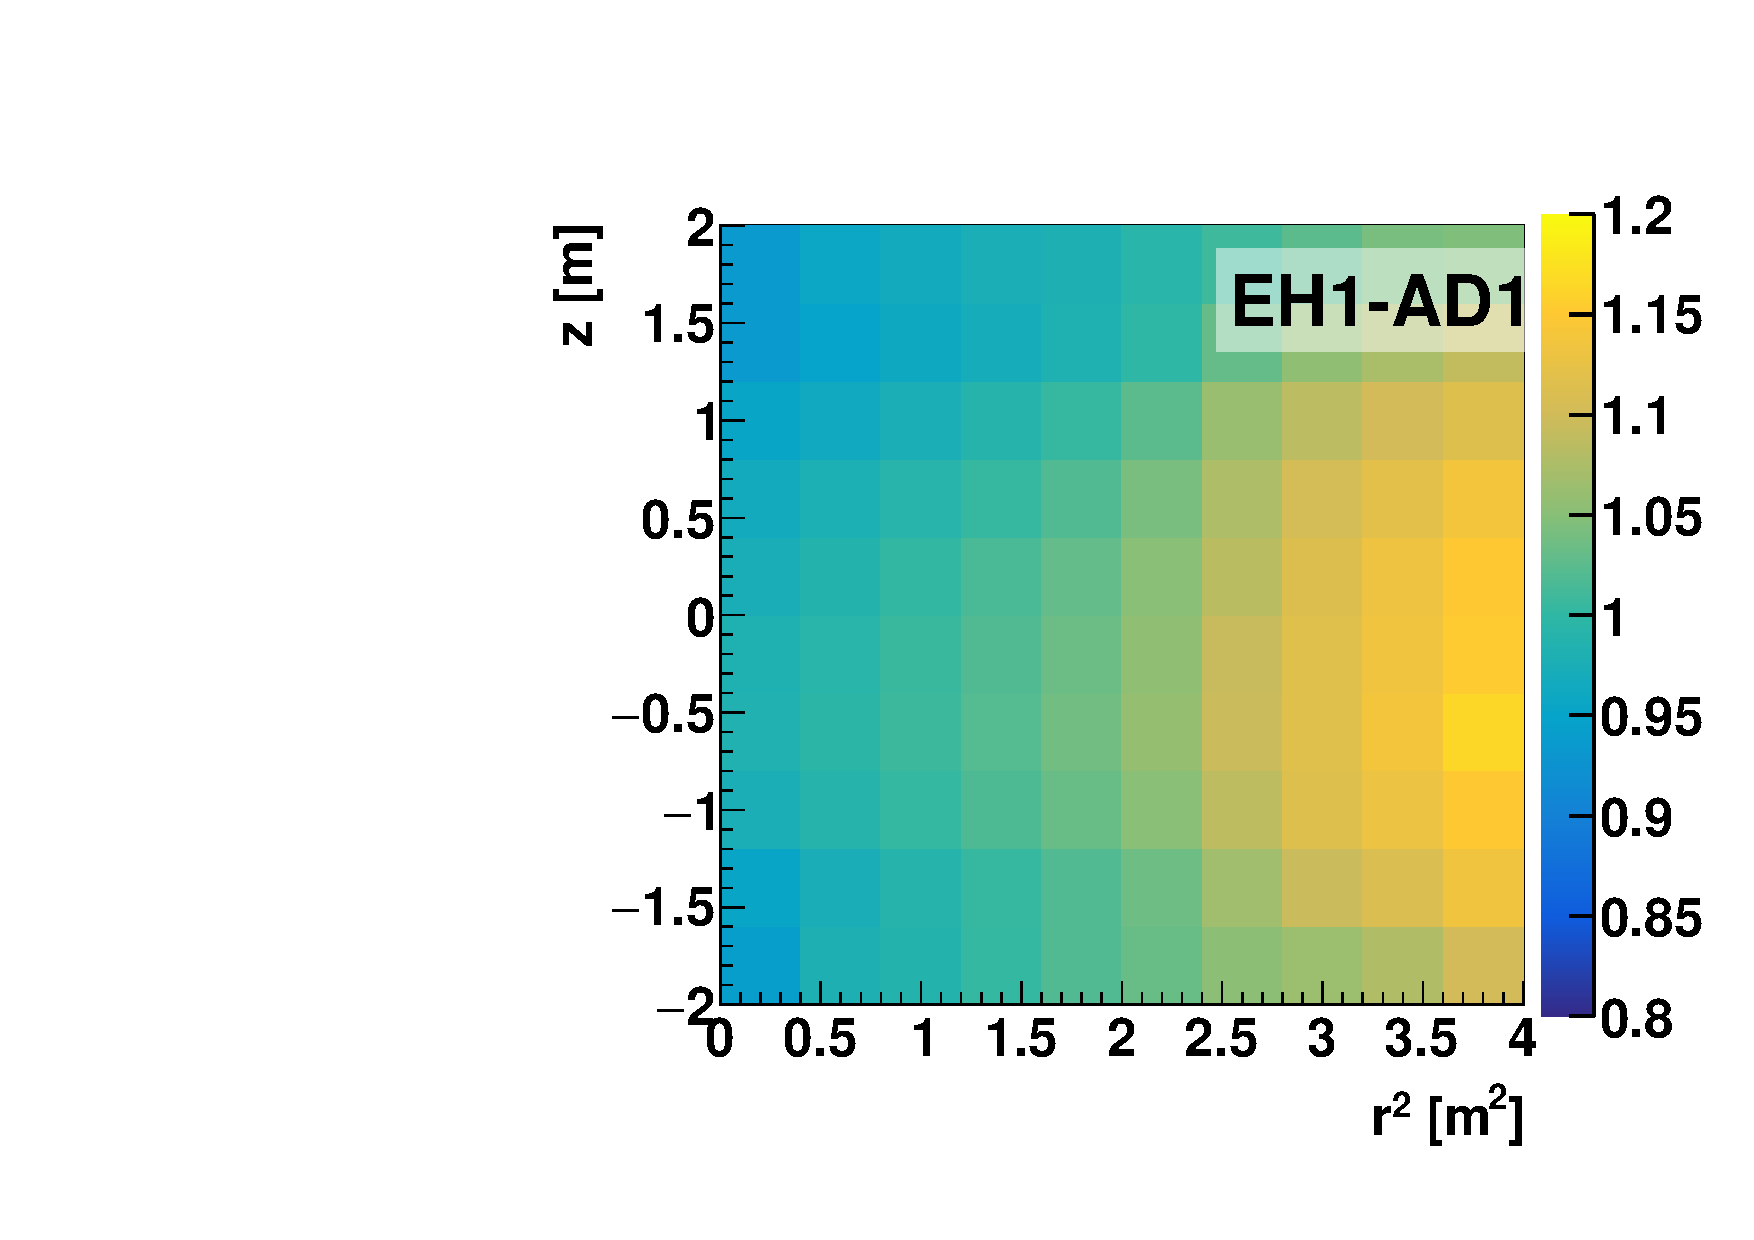
\includegraphics[width=0.4\textwidth]{ch_reconstruction/nonuniformity_map}
    \caption[Nonuniformity corrections]{
        Nonuniformity corrections based on the energy of spallation neutrons
        capturing on Gd and H.
        Plot based on data from \cite{nonuniformity2}.
    }
    \label{fig:nonuniformity_map}
\end{figure}

The Earth's magnetic field caused a nonuniformity
as a function of azimuthal angle $\phi$ of approximately \SI{1}{\percent}.
This effect was correlated with the orientation of the PMTs with respect
to the geomagnetic field.
A model was constructed to account for this effect:
\begin{equation}
    f_{\text{pos}}(\phi) = 1 + \alpha\sin(\phi-\phi_0),
\end{equation}
where $\alpha$ and $\phi_0$ were determined from fitting to spallation neutron captures
in a similar fashion as with the $r$--$z$ nonuniformity.

Over time, the nonuniformity evolved in different regions of the ADs,
attributable mostly to a slight degradation in the attenuation length of the LS
and GdLS \cite{nonuniformity3}.
The evolution was quantified by examining the spallation neutron capture energy
as a function of radial position and time.
As shown in \cref{fig:time_dep_nonunif}, a clear linear change is visible
for each bin of radial position \cite{nonuniformity1}, which was parametrized as
\begin{equation}
    f_{\text{pos}}(t, r) = (\beta_0 + \beta_1r^2)t.
\end{equation}
All ADs showed a similar trend, so a combined fit was performed,
yielding the values
\begin{align}\label{eq:tdnu_params}
    \begin{split}
        \beta_0 &= \SI[per-mode=reciprocal]{-0.116}{\per\year} \\
        \beta_1 &= \SI[per-mode=reciprocal]{0.075}{\per\square\meter\per\year},
    \end{split}
\end{align}
corresponding to rates of change between
\SIlist[list-units=repeat,retain-explicit-plus]{-0.12;+0.4}{\percent} per year.

\begin{figure}
    \centering
    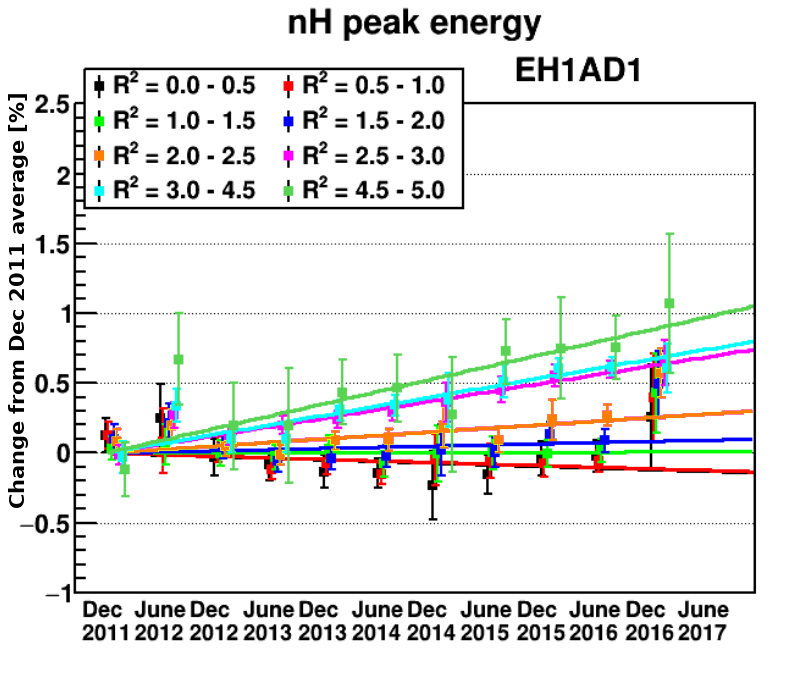
\includegraphics[width=0.8\textwidth]{ch_reconstruction/time_dep_nonunif_recolor}
    \caption[Time-dependent nonuniformity]{
        Relative change over time in energy for spallation neutrons capturing on H.
        Each color is a different range of event radius.
        The correction coefficients $\beta_0$ and $\beta_1$ are determined
        from a fit of the slope as a function of radius.
        Figure taken from \cite{nonuniformity4}.
    }
    \label{fig:time_dep_nonunif}
\end{figure}

\subsection{Energy resolution}
\label{subsec:resolution}

The detector energy resolution for a scintillating detector can be modeled as
\cite{energy_resolution}
\begin{equation}
    \frac{\sigma_E}{E} = \sqrt{a^2 + \frac{b^2}{E} + \frac{c^2}{E^2}},
\end{equation}
where $E$ is the reconstructed energy.
The parameters $a,b,$ and $c$ represent contributions to the resolution
from different sources.
Parameter $a$ quantifies the impact due to the non-pointlike nature
of the energy depositions in the scintillator,
since events with larger energy deposit their energy over a larger spatial extent
in the AD.
This could also be understood as a consequence of residual nonuniformity.
Parameter $b$ describes the size of the $\nicefrac{1}{\sqrt{E}}$ contribution,
which corresponds to the combined counting statistics of
the production, detection and digitization of photons.
Lastly, $c$ is a constant contribution to $\sigma_E$
representing the dark noise intrinsic to the PMTs.
The resolution parameters can be extracted from a fit
to the energy resolutions of a wide variety of calibration and intrinsic sources,
as shown in \cref{fig:resolution}.
The values for the resolution parameters are \cite{ngd2016}
\begin{align}\label{eq:resolution_params}
    \begin{split}
        a &= 0.016 \\
        b &= \SI{0.081}{\MeV\tothe{1/2}} \\
        c &= \SI{0.026}{\MeV}.
    \end{split}
\end{align}

\begin{figure}
    \centering
    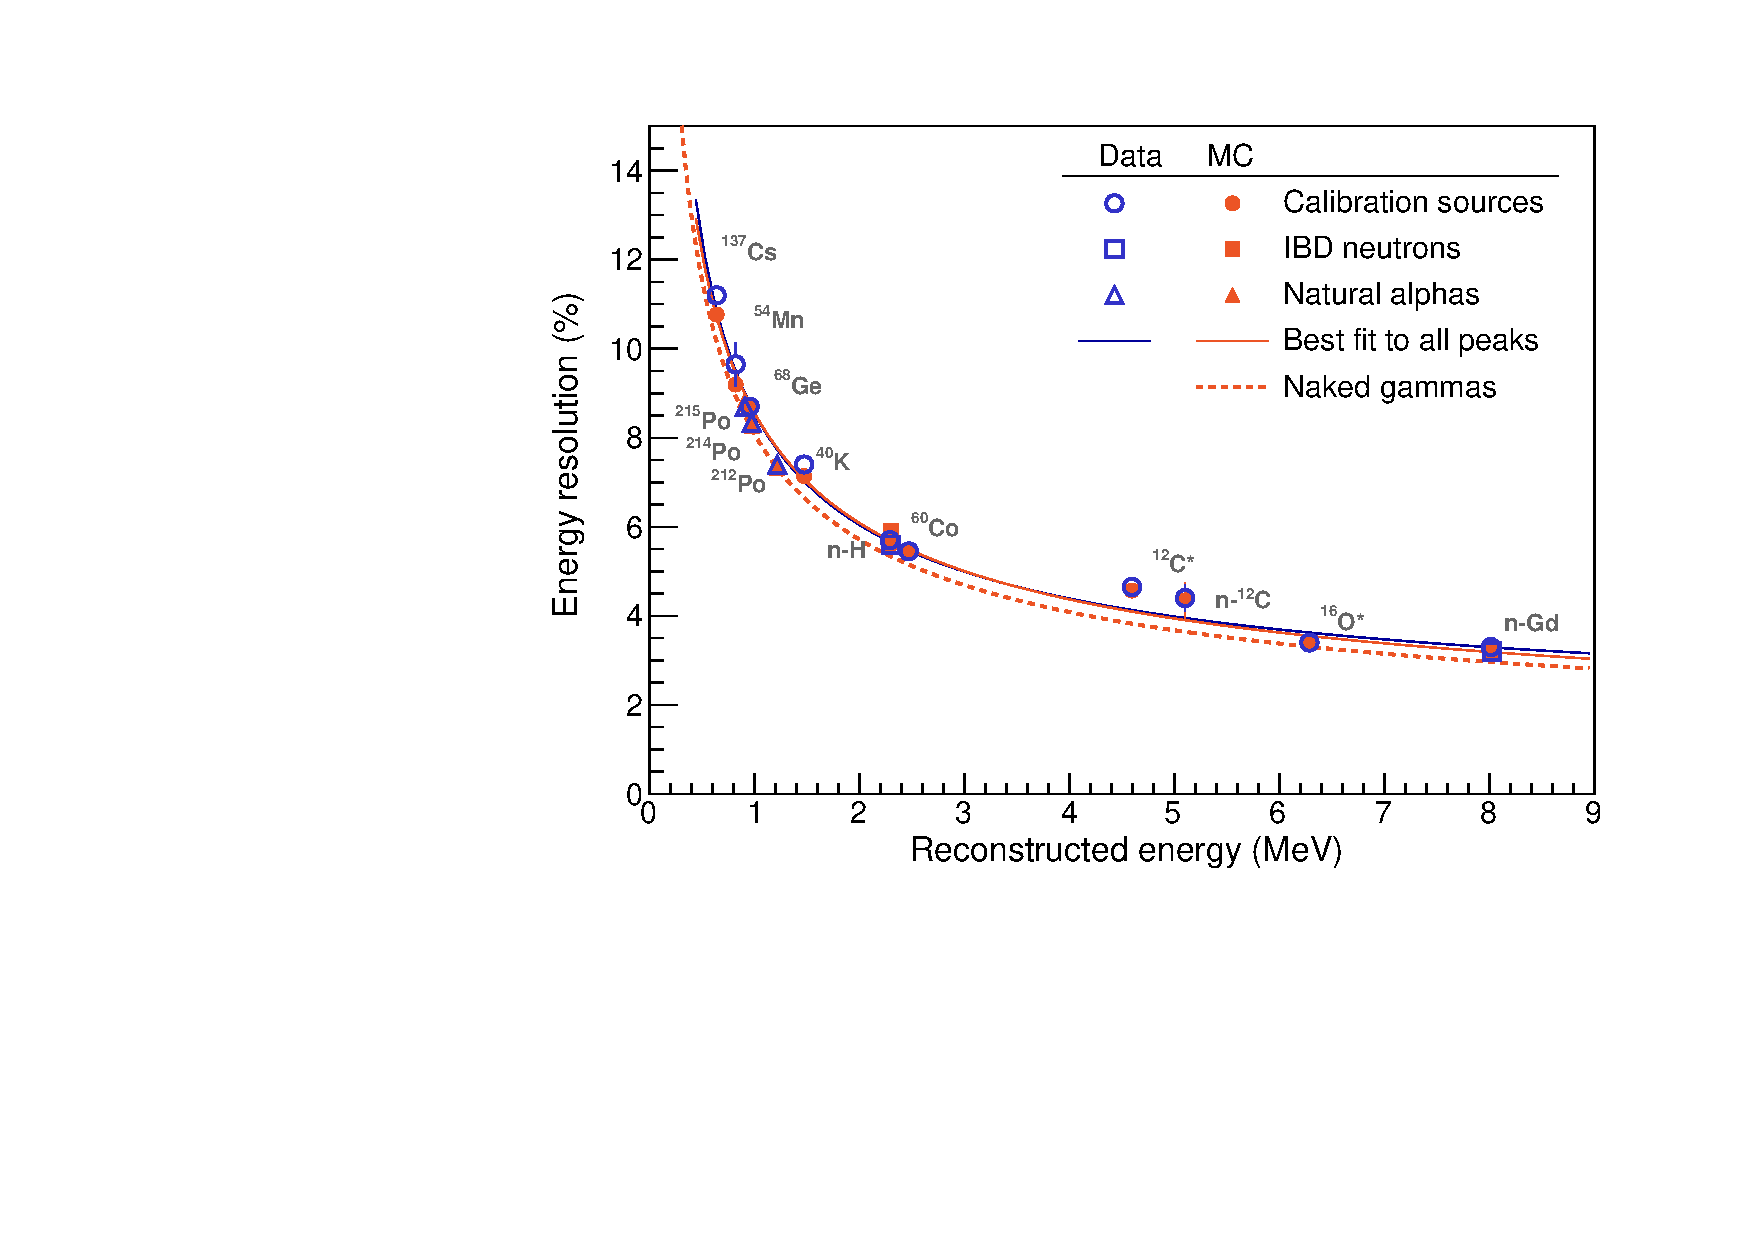
\includegraphics[width=0.8\textwidth]{ch_reconstruction/energy_resolution}
    \caption[Energy resolution]{Energy resolutions for calibration sources, neutron captures,
        and natural $\alpha$'s present in the ADs \cite{ngd2016}.
        The dashed orange line shows the simulated impact
        of optical shadowing (\cref{sec:special_calib}).
    }
    \label{fig:resolution}
\end{figure}


\subsection{Relative energy scale}
\label{subsec:rel_energyscale}

It was critical that all ADs measured the same energy when observing the same process.
If an AD had been biased and returned a higher or lower energy than the others,
then the IBD selection efficiency and spectral shape for that AD
could be different than at the other ADs,
which would bias the measurement of \thetaot{} and $\Delta m^2_{32}$.
The identicalness of the energy measurements is known as the relative energy scale,
and it was determined by measuring the same process in all ADs and comparing
the reconstructed energy.
The energy scale of the GdLS region was extremely well-constrained
by a thorough review of 13 calibration and intrinsic sources:
$\gamma$-rays from \isotope[68]{Ge} and \isotope[60]{Co} calibration sources;
neutron captures on Gd and H from both IBD and muon spallation;
$\alpha$ decays of naturally-occuring \isotope[212]{Po},
\isotope[214]{Po}, \isotope[215]{Po}, and \isotope[219]{Po};
and $\gamma$-rays from \isotope[40]{K} and \isotope[208]{Tl}.
\Cref{fig:gdls_rel_energyscale} shows the relative variations
for all of these sources among the 8 ADs.
The variations are all within \SI{+-0.2}{\percent}.

\begin{figure}
    \centering
    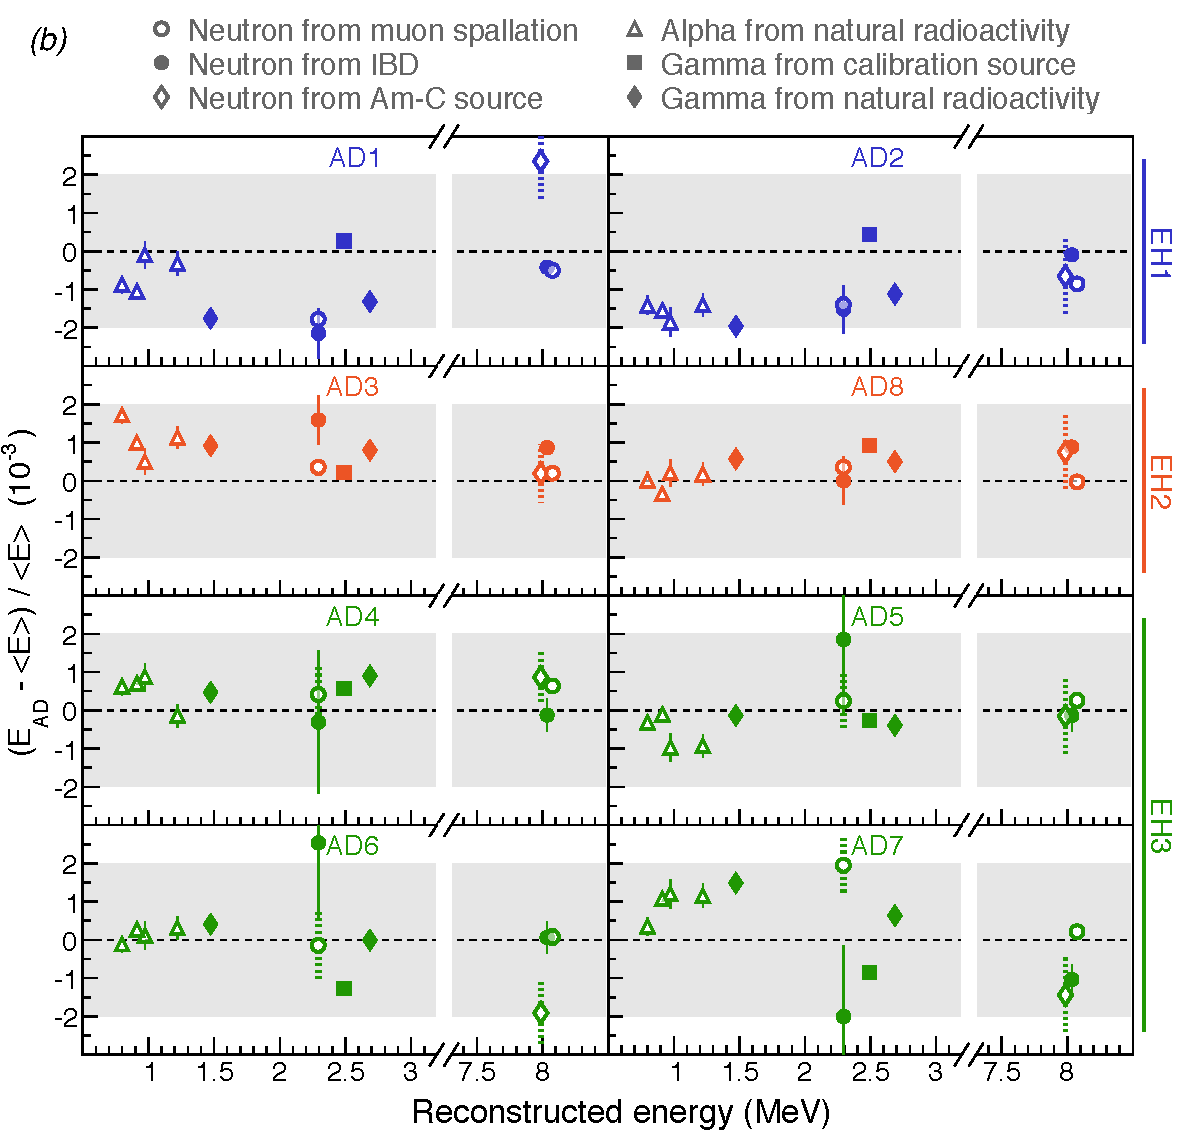
\includegraphics[width=0.9\textwidth]{ch_reconstruction/relative_energyscale}
    \caption[Relative energy scale for GdLS volume]{
        Comparison of 13 calibration and intrinsic source energies
        among the 8 ADs, showing the \SI{+-0.2}{\percent}
        relative energy scale variation in the GdLS region.
    }
    \label{fig:gdls_rel_energyscale}
\end{figure}

To include the LS region, the relative energy scale was studied
by comparing the energy of the neutron capture on H (nH)
among the ADs.
This technique is described in detail in \cref{subsec:delayed}
and resulted in a less-constrained relative energy scale variation
of \SI{+-0.5}{\percent}, which is conservatively adopted
as the energy scale uncertainty over the entire AD.
The impact of this variation on the prompt energy cut efficiency
and the prompt spectrum shape
was studied using simulation
as described in \cref{sec:thu_toymc}.

\subsection{Absolute energy scale}
\label{subsec:abs_energyscale}

The calibration and reconstruction procedures discussed so far
only ensured that the ADs have nearly-identical energy responses,
and that they all assigned the lower-energy $\gamma$-ray peak from nGd capture
to have energy \SI{7.95}{\MeV}.
Missing from the characterization is whether any other physical process
was assigned an accurate energy by the ADs.
That is, even if all ADs observing the same process
measured the same value $E_{\text{rec}}$
when the process had true energy $E_{\text{true}}$,
how close is $E_{\text{rec}}$ to $E_{\text{true}}$?
This question is particularly important when measuring the IBD prompt event energy,
which was used to determine the original \nuebar{} energy $E_\nu$
used to compute the survival probability (\cref{eq:p_sur_ee}).
The deviation as a function of $E_{\text{true}}$ is known as
the absolute energy scale or the absolute energy nonlinearity.

The absolute energy scale deviated from unity due to four main effects:
the IBD neutron recoil kinetic energy, scintillator quenching,
Cherenkov radiation, and electronics nonlinearity \cite{ngd2016}.
The effects were factored into electronics nonlinearities
and nonlinearities in generating detectable light signals
(i.e. visible energy, $E_{\text{vis}}$):
\begin{align}
    \begin{split}
        \frac{E_{\text{rec}}}{E_{\text{true}}}
        &=
        \frac{E_{\text{rec}}}{E_{\text{vis}}}
        \frac{E_{\text{vis}}}{E_{\text{true}}} \\
        &= \beta f_{\text{electronics}}(E_{\text{vis}})
        f_{\text{scintillator}}(E_{\text{true}}),
    \end{split}
\end{align}
with neutrons, quenching, and Cherenkov radiation contributing to
$f_{\text{scintillator}}(E_{\text{true}})$,
and the arbitrary normalization $\beta$ defined so that
$E_{\text{rec}} = E_{\text{true}}$
at the nGd capture peak reference energy of \SI{7.95}{\MeV}.
The electronics nonlinearity was applied on an event-by-event basis
through the single channel nonlinearity correction (see \cref{subsec:scnl}).
The scintillator nonlinearity was not applied to individual events;
instead, it was factored into the interaction and detector response model
applied to the binned data during the \thetaot{} fit procedure,
as described in \cref{ch:analysis}.

The neutron recoil energy was correlated with the \nuebar{} energy,
but did not result in any scintillation or Cherenkov light.
Fortunately, the energy lost was on the order of a few \si{\keV}
so was accepted as a slight broadening of the energy resolution.

The remaining scintillator effects were modeled for electrons as
\begin{equation}
    f_{\text{scintillator}}(E_{\text{true}}) =
    f_q(E_{\text{true}};k_B) + k_Cf_C(E_{\text{true}}),
\end{equation}
where $f_q$ describes the scintillation light including the quenching effect,
$k_B$ is Birks's constant which characterizes the medium (LS)
and particle type (electron),
$k_C$ is a normalization constant,
and $f_C$ is the Cherenkov light contribution.
For an electron which deposits all of its energy into the scintillator
with energy loss per unit length $\nicefrac{dE}{dx}$,
Birks's law determines the produced scintillation light up to normalization \cite{birks}:
\begin{equation}
    f_q(E_{\text{true}});k_B) = \frac{1}{E_{\text{true}}} \int_0^{E_{\text{true}}}
    \frac{dE}{1+k_B\frac{dE}{dx}}.
\end{equation}
The Cherenkov contribution $f_C$ was determined using a Monte Carlo simulation,
and $k_C$ was chosen so that the proportion of scintillation to Cherenkov photons
was correct at $E_{\text{true}} = \SI{1}{\MeV}$.
These results were then converted for use by positrons under the assumption that
(a) electrons and positrons have identical scintillation and Cherenkov properties;
and (b) on annihilation, two additional \SI{0.511}{\MeV} $\gamma$-rays are emitted.
These $\gamma$'s as well as $\gamma$'s produced by nH, nGd and other processes
can be treated recursively
since they lose energy in the scintillator
by Compton scattering, the photoelectric effect, and pair-conversion,
and the $e^{\pm}$ generated from these processes
are described by $f_{\text{scintillator}}$.
\Cref{fig:gamma_conversion} shows the probability distributions
of the energy of $e^{\pm}$ generated by a $\gamma$-ray
and subsequent electromagnetic shower for various $\gamma$ energies,
which were used to produce effective nonlinearity models for $\gamma$-rays.

\begin{figure}
    \centering
    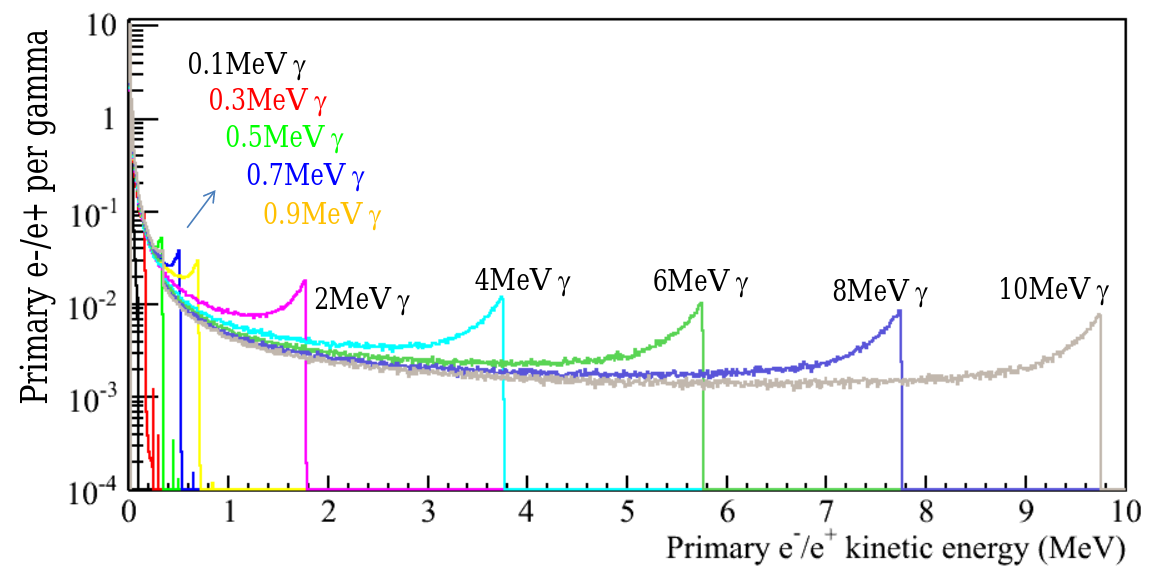
\includegraphics[width=0.9\textwidth]{ch_reconstruction/gamma_conversion_energy}
    \caption[$e^{\pm}$ spectrum from $\gamma$-rays]{
        Probability for a $\gamma$-ray of a given energy to produce
        an $e^{\pm}$ with a given energy in Daya Bay liquid scintillator.
        This plot was produced using Monte Carlo and is taken from \cite{nonlinearity1}.
    }
    \label{fig:gamma_conversion}
\end{figure}

\subsection{Single channel non-linearity correction}
\label{subsec:scnl}

The electronics used to digitize the PMT signals had intrinsic non-linearities,
dominated by the summing circuit's performance
when faced with multiple overlapping PMT signals.
To precisely characterize the performance of the electronics,
a dedicated 192-channel flash analog-to-digital converter (FADC) system
was installed in EH1-AD1 in December 2015
with the ability to digitize the raw PMT waveforms at \SI{1}{\GHz} \cite{scnl_technote}.
\Cref{fig:fadc_schematic} shows the integration of the FADC system
with the existing front-end electronics (FEE).
Specifically, the FADC received copies of each PMT's HV-decoupled signal,
amplified by a factor of 10,
along with the clock and trigger signals issued by the FEE.
Thus the FADC was able to record individual PMT waveforms
without the nonlinearity effects faced by the FEE.

\begin{figure}
    \centering
    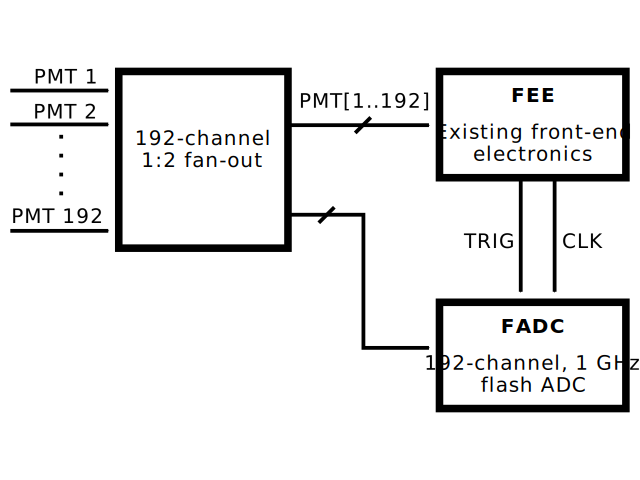
\includegraphics[width=0.6\textwidth]{ch_reconstruction/fadc_schematic}
    \caption[FADC schematic]{
        Schematic showing the integration of the FADC
        with the existing FEE system.
        Based on \cite{scnl_poster}.
    }
    \label{fig:fadc_schematic}
\end{figure}

These FADC waveforms were compared event-by-event and channel-by-channel
to the records produced by the FEE as a ratio, $Q_\text{FEE}/Q_\text{FADC}$,
as shown in \cref{fig:scnl_by_event}.
A single curve was produced for each channel by taking the average ratio
for a given bin of FADC charge.
The results for each channel, as well as the average over all channels,
is shown in \cref{fig:scnl_by_channel}.
Variation among channels was limited to an RMS of \SI{1}{\percent}.

Higher-energy events and those located near the edge of the AD
tended to produce charge signals on some PMTs which
saturated their FADC channels due to the amplification factor of 10.
Saturated channels were excluded from the computation of the nominal nonlinearity curve,
so a second approach was required to ensure the result was accurate
for channels with $\gtrsim \SI{10}{\pe}$.
A second nonlinearity curve, shown in \cref{fig:scnl_low_gain},
was generated using a smaller amplification factor of 4 for the input to the FADC
to reduce the effect of the saturated channels \cite{scnl_slides}.

The two nonlinearity curves (high-gain and low-gain) were used
to construct a table of corrections
that converted the measured FEE charge on each channel
to the average charge measured for similar events by the FADC.
This correction was applied independently to each channel
and was known as the ``single-channel nonlinearity correction'' or SCNL.
The correction values are displayed as a curve in \cref{fig:scnl_correction};
the correction was applied as
\begin{equation}\label{eq:scnl}
    f_\text{SCNL}(N_\text{obs,\,FEE}) = \frac{N_\text{obs,\,FEE}}{\text{FEE/FADC}},
\end{equation}
where FEE/FADC is the correction value from \cref{fig:scnl_correction}.
A residual nonlinearity of \SI{0.5}{\percent}
was attributed to the large event-by-event variations
from the average (correction) value,
especially when the charge on a channel was $\lesssim\SI{1}{\pe}$.
The residual nonlinearity for a single channel is shown in \cref{fig:scnl_residual}.

\begin{figure}
    \centering
    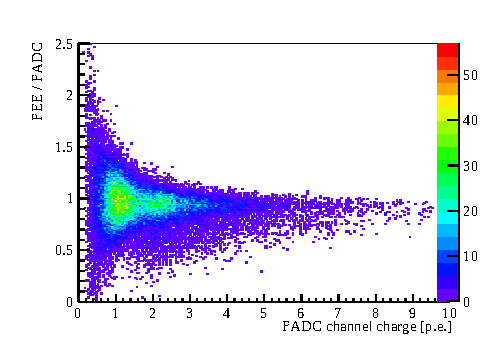
\includegraphics[width=0.7\textwidth]{ch_reconstruction/scnl_by_event}
    \caption[Flash ADC comparison to FEE, event by event]{
        Comparison of the extracted charge for a single PMT channel
        (EH1-AD1, row 2, column 6)
        over many events.
        The vertical axis represents the ratio of the FEE-recorded charge
        to the FADC-recorded charge for this channel.
        Figure taken from \cite{scnl_technote}.
    }
    \label{fig:scnl_by_event}
\end{figure}

\begin{figure}
    \centering
    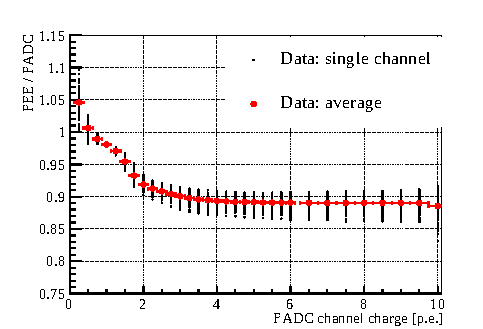
\includegraphics[width=0.7\textwidth]{ch_reconstruction/scnl_by_channel}
    \caption[Flash ADC comparison to FEE, channel by channel]{
        Average ratio of FADC charge to FEE charge for each channel (black),
        along with the average over all channels (red).
        Figure taken from \cite{scnl_technote}.
    }
    \label{fig:scnl_by_channel}
\end{figure}

\begin{figure}
    \centering
    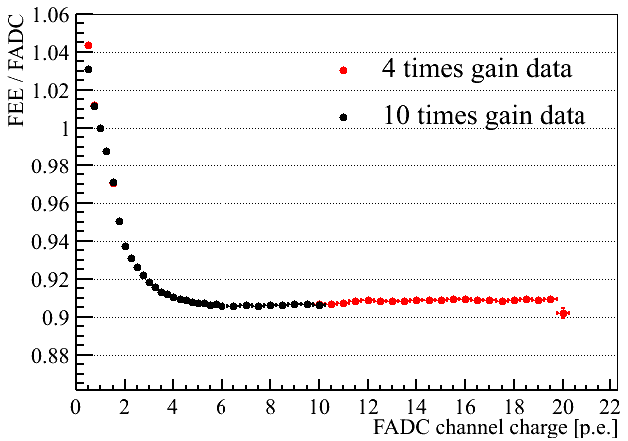
\includegraphics[width=0.7\textwidth]{ch_reconstruction/scnl_low_gain}
    \caption[Flash ADC comparison to FEE, low gain]{
        Nonlinearity curves from the high-gain (factor of 10, black)
        and the low-gain (factor of 4, red)
        FADC data runs.
        Figure taken from \cite{scnl_slides}.
    }
    \label{fig:scnl_low_gain}
\end{figure}

\begin{figure}
    \centering
    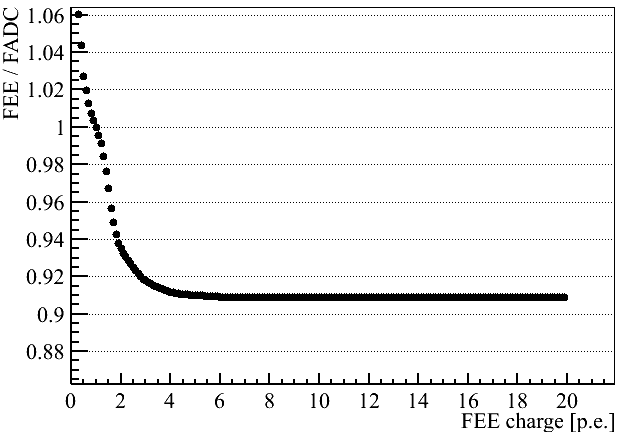
\includegraphics[width=0.7\textwidth]{ch_reconstruction/scnl_correction}
    \caption[SCNL: final correction curve]{
        Single-channel nonlinearity (SCNL) correction
        as a function of observed FEE charge.
        Figure taken from \cite{scnl_technote}.
    }
    \label{fig:scnl_correction}
\end{figure}

\begin{figure}
    \centering
    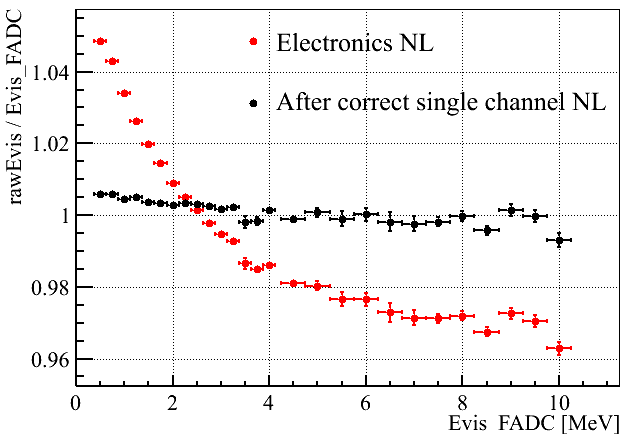
\includegraphics[width=0.7\textwidth]{ch_reconstruction/scnl_residual}
    \caption[SCNL: residual nonlinearity]{
        Observed single-channel nonlinearity before (red) and after (black)
        the SCNL correction.
        Figure taken from \cite{scnl_technote}.
    }
    \label{fig:scnl_residual}
\end{figure}
